\documentclass[12pt]{article}
%%%%%%%%%%%%%%%%%%%%%%%%%%%%%%%%%%%%%%%%%

\usepackage{amscd}
\usepackage{amsmath}
\usepackage{amssymb}
\usepackage{amsthm}
\usepackage{ulem}
\usepackage{epsfig}
\usepackage{verbatim}
\usepackage{graphicx}
\usepackage{amsthm}
\pagestyle{empty}
\usepackage{color}
\usepackage{hyperref}

\setlength{\textheight}{8.5in} \setlength{\topmargin}{0.0in}
\setlength{\headheight}{0.0in} \setlength{\headsep}{0.0in}
\setlength{\leftmargin}{0.5in}
\setlength{\oddsidemargin}{0.0in}
%\setlength{\parindent}{1pc}
\setlength{\textwidth}{6.5in}
%\linespread{1.6}

\newtheorem{definition}{Definition}
\newtheorem{problem}{Problem}

\newtheorem{theorem}{Theorem}[section]
\newtheorem{lemma}[theorem]{Lemma}
\newtheorem{note}[theorem]{Note}
\newtheorem{corollary}[theorem]{Corollary}
\newtheorem{prop}[theorem]{Proposition}

%%%%%%%%%%%%%%%%%%%%%%%%%%%%%%%%%%%%%%%%%

\begin{document}
\thispagestyle{empty}

\bigskip
\bigskip

\centerline{\textbf{\Large{ENPM 808M - Project Pre-Proposal}}}

\bigskip
\bigskip


\noindent \textbf{Name:} %Your name goes here.
Kanishka Ganguly and Kiran Yakkala

\bigskip

\noindent \textbf{Major:} %Write your majors, minors or GECs.
Professional Masters in Robotics

\bigskip 

\noindent \textbf{Proposed Topic:} %Write a brief description of the topic you wish to work on. This should be done in 40 words or less. 
We propose to create a model of an anthropomorphic gripper, with four fingers and a thumb. This model could be used for dexterous gripping actions that most industrial grippers are not capable of currently.

\bigskip

\noindent \textbf{Advisor:} %Write the name of any professor(s) you think you might want to work with on this topic. You may leave this section blank if you don't know. 
Dr. William S. Levine

\bigskip

\section*{Proposal}
In this project, we aim to model and simulate a basic anthropomorphic gripper, based on four fingers and a thumb. Note that we do not attempt to model the gripper biomimetically.\\
Most common industrial grippers have two or three gripping surfaces which are useful when `top-down' gripping is required. However, for a more dexterous approach at gripping objects, a more natural gripping solution is required.\\
The human hand is capable of 27 degrees of freedom, including the rotation and translation of the wrist.\cite{dof} Here we aim to model only the 19 degrees of freedom provided by the fingers and thumb only.\\
\newline
\begin{figure}[h!]
\caption{Bones in Human Hand}
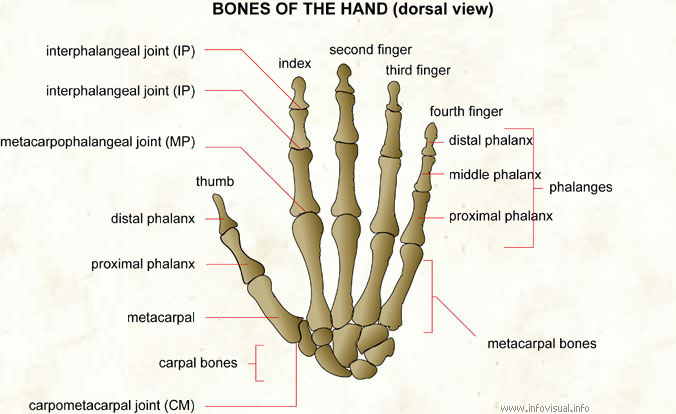
\includegraphics[scale=1.5]{img/finger_names.jpg}
\label{fig:bones}
\centering
\end{figure}
\begin{itemize}
\item \uuline{Fingers} (4 DOF each)\\
As seen in figure \ref{fig:bones}, each finger has a joint between the distal and the middle phalange and a joint between the middle and the proximal phalange. These allow extension/flexion (2 DOF).\\
There is also a joint between the proximal phalange and the metacarpal that allows for abduction/adduction along with the standard flexion/extension (2 DOF).

\item \uuline{Thumbs} (5 DOF)\\
The thumb has an interphalangeal joint between the distal and proximal phalanges allowing flexion/extension (1 DOF); a metacarpophalangeal joint between the proximal phalanx and metacarpal allowing flexion/extension and abduction/adduction (2 DOF); a carpometacarpal joint between the metacarpal and trapezium allowing flexion/extension and abduction/adduction (2 DOF).\\
Out of these 5 degrees of freedom, we aim to model only 3, namely the joints between distal and proximal phalanges and the joint between proximal phalanx and metacarpal.
\end{itemize}

Now, consider the following diagram for a model of the anthropomorphic gripper.\cite{model}
\begin{figure}[h!]
\caption{Model of Hand}
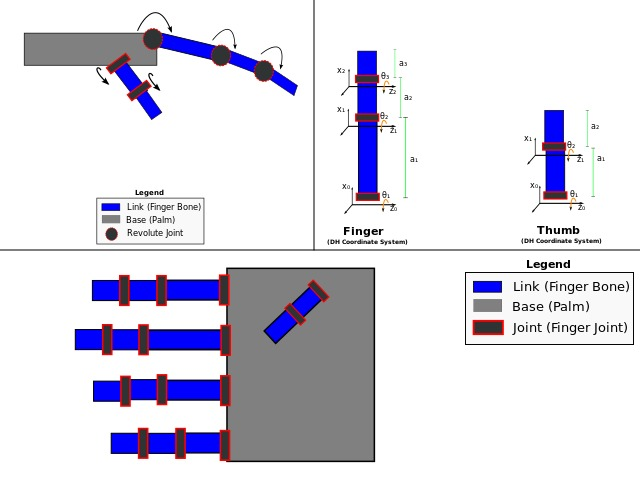
\includegraphics[scale=0.5]{img/hand_diagram.jpg}
\label{fig:diagram}
\centering
\end{figure}
\vspace{20pt}
\begin{figure}[h!]
\caption{3D Model of Hand}
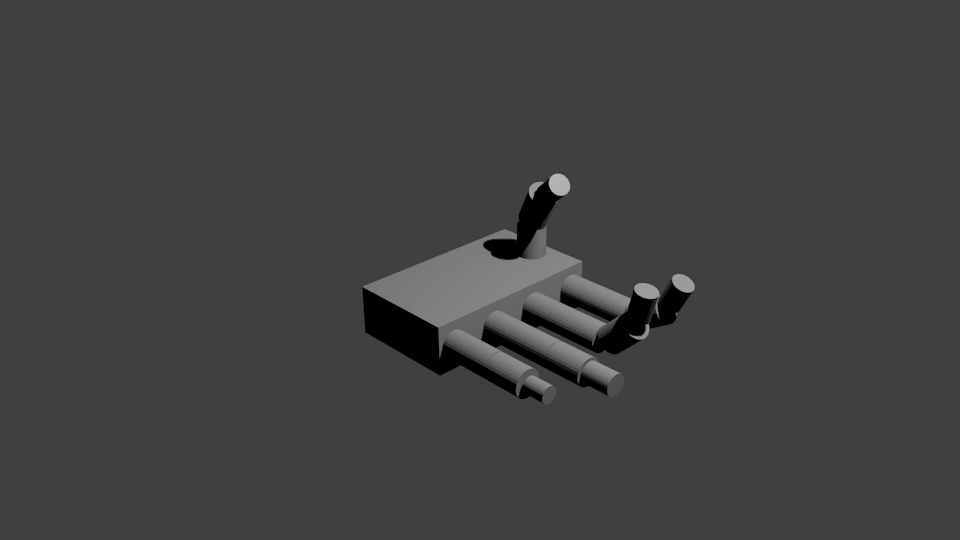
\includegraphics[scale=0.21]{img/3dhand.png}
\label{fig:3d}
\centering
\end{figure}

From Figure \ref{fig:diagram}, we propose the following DH parameters for the anthropomorphic gripper:
\begin{itemize}
\item
\uuline{Fingers}\\
\begin{center}
\begin{tabular}{|l|l|l|l|l|{c}r}
\hline
Link ($i$) & $a_i$ & $\alpha_i$ & $d_i$ & $\theta_i$\\
\hline
1 & $a_1$ & $0$ & $0$ & $\theta_1$\\
2 & $a_2$ & $0$ & $0$ & $\theta_2$\\
3 & $a_3$ & $0$ & $0$ & $\theta_3$\\
\hline
\end{tabular}
\end{center}

\item
\uuline{Thumb}\\
\begin{center}
\begin{tabular}{|l|l|l|l|l|{c}r}
\hline
Link ($i$) & $a_i$ & $\alpha_i$ & $d_i$ & $\theta_i$\\
\hline
1 & $a_1$ & $0$ & $0$ & $\theta_1$\\
2 & $a_2$ & $0$ & $0$ & $\theta_2$\\
\hline
\end{tabular}
\end{center}
\end{itemize}

Given these parameters, we can aim to find the forward kinematic equations for each of the finger tips. Also, since we are assuming each finger to be its own kinematic chain, we can get precise control over the motion of each finger, independent of each other.\\

\section*{Further Scope}
At a later stage in the project, we aim to add a `sideways' motion to the base of each finger as well, as can be seen in a human hand.\\
Also, we can attach the gripper to the end of a generic Stanford Arm to fully realize the range of motion provided by an actual human hand.
\bigskip

\section*{Tentative Timeline}
\uuline{Goal I (Minimum Objective)}\\
\textbf{Modelling of basic 14 DOF hand, including IK calculations for the same.}\\
\begin{itemize}
\item \textit{\uline{Nov. 1, 2015 - Nov. 15, 2015}}\\
CAD Model and 3D Animation
\item \textit{\uline{Nov. 16, 2015 - Nov. 30, 2015}}\\
Inverse kinematics calculations\\
SimMechanics Simulation
\end{itemize}

\uuline{Goal II (Intermediate Objective)}\\
\textbf{Adding remaining 5 degrees of freedom, through `sideways' motion of thumb and fingers}\\
\begin{itemize}
\item \textit{\uline{Dec. 1, 2015 - Dec. 10, 2015}}\\
Inverse kinematics calculations\\
SimMechanics Simulation
\end{itemize}

\uuline{Goal III (Final Objective)}\\
\textbf{Integration with Stanford Arm}\\
\begin{itemize}
\item \textit{\uline{Dec. 11, 2015 - Dec. 19, 2015}}\\
CAD Modelling\\
Inverse kinematics calculations\\
SimMechanics Simulation
\end{itemize}

\bigskip

\section*{Note}
Considering the complexity of this project and the ambitious but achievable target, we hope to finish the entire project by the $19^{th}$ of December, 2015.\\
However, we are setting the final goal on standby, to be attempted if time permits us and the other two goals are completed satisfactorily.\\
The main reason for this being that the aim of this project is to model and simulate the motion of the human fingers as a gripper and not the entire arm itself.

\begin{thebibliography}{9}

\bibitem{dof} StackOverflow. \url{http://biology.stackexchange.com/questions/30857/does-the-human-hand-have-27-degrees-of-freedom}
\bibitem{model} Modelling and Control for Soft Finger Manipulation and Human-Robot Interaction. \textit{Fanny Ficuciello}, \url{http://wpage.unina.it/fanny.ficuciello/files/Thesis_ficuciello.pdf}
\end{thebibliography}

%%%%%%%%%%%%%%%%%%%%%%%%%%%%%%%%%%%%%%%%%
\end{document} 
